\documentclass[11pt,a4paper]{article}

% ============================================================================
% PACKAGES
% ============================================================================
\usepackage[utf8]{inputenc}
\usepackage[T1]{fontenc}
\usepackage{geometry}
\usepackage{graphicx}
\usepackage{booktabs}
\usepackage{amsmath}
\usepackage{amssymb}
\usepackage{hyperref}
\usepackage{xcolor}
\usepackage{listings}
\usepackage{float}
\usepackage{caption}
\usepackage{subcaption}
\usepackage{enumitem}
\usepackage{fancyhdr}
\usepackage{tikz}
\usepackage{pgfplots}
\usepackage{multicol}
\usepackage{algorithm}
\usepackage{algpseudocode}
\usepackage{longtable}
\usepackage{pifont}
\usepackage{tocloft}
\usepackage[numbers,sort&compress]{natbib}
\pgfplotsset{compat=1.17}
\usetikzlibrary{shapes,arrows,positioning}

% Graphics path for images
\graphicspath{{../outputs/plots/}{../outputs/rules/}{../outputs/gephi/}}

% ============================================================================
% PAGE SETUP
% ============================================================================
\geometry{margin=1in}
\setlength{\parindent}{0pt}
\setlength{\parskip}{0.5em}

% Header/Footer
\pagestyle{fancy}
\fancyhf{}
\rhead{MetaFam Knowledge Graph}
\lhead{Precog Research Task}
\rfoot{Page \thepage}

% Colors
\definecolor{codegreen}{rgb}{0,0.6,0}
\definecolor{codegray}{rgb}{0.5,0.5,0.5}
\definecolor{codepurple}{rgb}{0.58,0,0.82}
\definecolor{backcolour}{rgb}{0.95,0.95,0.92}
\definecolor{highconf}{HTML}{55A868}
\definecolor{medconf}{HTML}{F5A623}
\definecolor{lowconf}{HTML}{C44E52}
\definecolor{task1}{HTML}{3498DB}
\definecolor{task2}{HTML}{E74C3C}
\definecolor{task3}{HTML}{2ECC71}
\definecolor{task4}{HTML}{9B59B6}

% Hyperref setup
\hypersetup{
    colorlinks=true,
    linkcolor=blue,
    filecolor=magenta,
    urlcolor=cyan,
}

% ============================================================================
% DOCUMENT
% ============================================================================
\begin{document}

% ----------------------------------------------------------------------------
% TITLE PAGE
% ----------------------------------------------------------------------------
\begin{titlepage}
    \centering
    \vspace*{1cm}
    
    {\Huge\bfseries MetaFam Knowledge Graph\\[0.3cm]Complete Analysis Report\par}
    
    \vspace{1cm}
    
    {\Large\textit{``Happiness can be found even in the darkest of times,\\if only one remembers to turn on the light''}\par}
    {\large --- Albus Dumbledore\par}
    
    \vspace{1.5cm}
    
    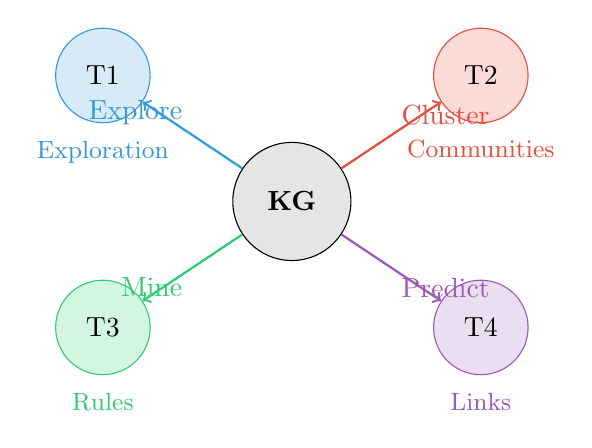
\begin{tikzpicture}[scale=0.8]
        % Central node
        \node[circle, draw=black, fill=gray!20, minimum size=1.5cm] (kg) at (0,0) {\textbf{KG}};
        
        % Task nodes
        \node[circle, draw=task1, fill=task1!20, minimum size=1.2cm] (t1) at (-3,2) {T1};
        \node[circle, draw=task2, fill=task2!20, minimum size=1.2cm] (t2) at (3,2) {T2};
        \node[circle, draw=task3, fill=task3!20, minimum size=1.2cm] (t3) at (-3,-2) {T3};
        \node[circle, draw=task4, fill=task4!20, minimum size=1.2cm] (t4) at (3,-2) {T4};
        
        % Connections
        \draw[->, thick, task1] (kg) -- (t1) node[midway, above left] {Explore};
        \draw[->, thick, task2] (kg) -- (t2) node[midway, above right] {Cluster};
        \draw[->, thick, task3] (kg) -- (t3) node[midway, below left] {Mine};
        \draw[->, thick, task4] (kg) -- (t4) node[midway, below right] {Predict};
        
        % Labels
        \node[below=0.1cm of t1, task1] {\small Exploration};
        \node[below=0.1cm of t2, task2] {\small Communities};
        \node[below=0.1cm of t3, task3] {\small Rules};
        \node[below=0.1cm of t4, task4] {\small Links};
    \end{tikzpicture}
    
    \vspace{1.5cm}
    
    {\Large\textbf{Precog Research Task}\par}
    \vspace{0.5cm}
    {\large Knowledge Graph Analysis \& Machine Learning\par}
    
    \vspace{1cm}
    
    \begin{tabular}{rl}
        \textbf{Task 1:} & Dataset Exploration \\
        \textbf{Task 2:} & Community Detection \\
        \textbf{Task 3:} & Rule Mining \\
        \textbf{Task 4:} & Link Prediction \\
    \end{tabular}
    
    \vfill
    
    {\large February 2026\par}
\end{titlepage}

% ----------------------------------------------------------------------------
% TABLE OF CONTENTS
% ----------------------------------------------------------------------------
\tableofcontents
\newpage

% ----------------------------------------------------------------------------
% EXECUTIVE SUMMARY
% ----------------------------------------------------------------------------
\section{Executive Summary}

This report presents a comprehensive analysis of the \textbf{MetaFam Knowledge Graph}, a synthetic family network dataset. The analysis spans four interconnected tasks that progressively build understanding from basic exploration to advanced machine learning.

\subsection{Dataset Overview}

\begin{table}[H]
    \centering
    \caption{MetaFam Dataset Statistics}
    \begin{tabular}{lc}
        \toprule
        \textbf{Metric} & \textbf{Value} \\
        \midrule
        Total Nodes (Entities) & 1,316 \\
        Total Edges (Triples) & 13,821 \\
        Unique Relation Types & 28 \\
        Connected Components & 50 \\
        Average Degree & 21.0 \\
        Graph Density & 0.008 \\
        \bottomrule
    \end{tabular}
\end{table}

\subsection{Key Findings Across Tasks}

\begin{enumerate}
    \item \textbf{Task 1 (Exploration):} MetaFam is a forest of 50 isolated family trees, each spanning 4 generations with balanced gender distribution (51\% female, 49\% male). High clustering coefficient (0.73) indicates strong family cohesion.
    
    \item \textbf{Task 2 (Communities):} All three algorithms (Girvan-Newman, Louvain, Leiden) achieved near-perfect modularity ($Q \approx 0.98$), detecting exactly 50 communities corresponding to the 50 family clusters.
    
    \item \textbf{Task 3 (Rules):} Discovered 8 horn-clause rules with varying confidence. Transitive rules (grandmother, sibling, aunt) achieved 100\% confidence. Complex cousin rules showed 0\% confidence due to missing relation types.
    
    \item \textbf{Task 4 (Link Prediction):} Implemented KGE models (TransE, DistMult, ComplEx, RotatE) and GNN approaches (RGCN) with three data splitting strategies to analyze data leakage and generalization.
\end{enumerate}

\subsection{Technical Contributions}

\begin{itemize}
    \item Comprehensive graph analysis pipeline with gender/generation inference
    \item Multiple community detection algorithms with comparative evaluation
    \item Horn-clause rule validation engine with noise analysis
    \item Link prediction framework with leakage-aware data splitting
\end{itemize}

% ============================================================================
% PART I: DATASET EXPLORATION (TASK 1)
% ============================================================================
\newpage
\part{Dataset Exploration}

\section{Introduction to Task 1}

The first task establishes the foundational understanding of the MetaFam knowledge graph through systematic exploration of its structure, metrics, and patterns.

\subsection{Objectives}

\begin{enumerate}
    \item Load and understand the dataset structure
    \item Compute graph metrics (density, clustering, centrality)
    \item Analyze node attributes (gender, generation)
    \item Extract qualitative insights about family network patterns
\end{enumerate}

\section{Graph Structure Analysis}

\subsection{Basic Statistics}

\begin{table}[H]
    \centering
    \caption{Fundamental Graph Properties}
    \begin{tabular}{lcc}
        \toprule
        \textbf{Property} & \textbf{Directed} & \textbf{Undirected} \\
        \midrule
        Nodes & 1,316 & 1,316 \\
        Edges & 13,821 & 6,910 \\
        Components (Weakly/Connected) & 50 & 50 \\
        Average Degree & 21.0 & 10.5 \\
        \bottomrule
    \end{tabular}
\end{table}

\subsection{Relationship Types}

The 28 unique relations are categorized into:

\begin{table}[H]
    \centering
    \caption{Relationship Categories}
    \begin{tabular}{ll}
        \toprule
        \textbf{Category} & \textbf{Relations} \\
        \midrule
        Parent-Child & fatherOf, motherOf, sonOf, daughterOf \\
        Sibling & brotherOf, sisterOf \\
        Grandparent & grandfatherOf, grandmotherOf, grandsonOf, granddaughterOf \\
        Extended & uncleOf, auntOf, nephewOf, nieceOf \\
        Cousin & boyCousinOf, girlCousinOf \\
        Great-Relations & greatUncleOf, greatAuntOf, etc. \\
        \bottomrule
    \end{tabular}
\end{table}

\textbf{Notable Absence:} Spouse relations (husbandOf, wifeOf) are missing, explaining the 50 isolated family components.

\begin{figure}[H]
    \centering
    \includegraphics[width=0.85\textwidth]{relationship_distribution.png}
    \caption{Distribution of relationship types in the MetaFam knowledge graph. Parent-child and sibling relations dominate the dataset.}
    \label{fig:relation_dist}
\end{figure}

\subsection{Network Metrics}

\begin{table}[H]
    \centering
    \caption{Key Network Metrics}
    \begin{tabular}{lcc}
        \toprule
        \textbf{Metric} & \textbf{Value} & \textbf{Interpretation} \\
        \midrule
        Density & 0.008 & Very sparse (typical for social networks) \\
        Avg. Clustering Coef. & 0.735 & High transitivity (family cohesion) \\
        Max Betweenness & 0.0001 & No bridge individuals \\
        \bottomrule
    \end{tabular}
\end{table}

\begin{figure}[H]
    \centering
    \includegraphics[width=0.75\textwidth]{degree_distribution.png}
    \caption{Degree distribution of nodes in the undirected MetaFam graph. The distribution shows the typical connectivity patterns within family structures.}
    \label{fig:degree_dist}
\end{figure}

\section{Node Attribute Analysis}

\subsection{Gender Distribution}

Gender was inferred from relation semantics (e.g., \texttt{fatherOf} $\rightarrow$ Male):

\begin{table}[H]
    \centering
    \begin{tabular}{lcc}
        \toprule
        \textbf{Gender} & \textbf{Count} & \textbf{Percentage} \\
        \midrule
        Female & 671 & 51.0\% \\
        Male & 645 & 49.0\% \\
        \bottomrule
    \end{tabular}
\end{table}

\begin{figure}[H]
    \centering
    \includegraphics[width=0.6\textwidth]{gender_distribution.png}
    \caption{Gender distribution inferred from relation semantics (e.g., fatherOf $\rightarrow$ Male). Near-equal split indicates balanced synthetic generation.}
    \label{fig:gender_dist}
\end{figure}

\subsection{Generational Structure}

\begin{table}[H]
    \centering
    \caption{Generation Distribution}
    \begin{tabular}{lccc}
        \toprule
        \textbf{Generation} & \textbf{Count} & \textbf{Percentage} & \textbf{Role} \\
        \midrule
        0 (Founders) & 100 & 7.6\% & Great-grandparents \\
        1 & 457 & 34.7\% & Grandparents \\
        2 & 750 & 57.0\% & Parents \\
        3 (Youngest) & 9 & 0.7\% & Children \\
        \bottomrule
    \end{tabular}
\end{table}

\begin{figure}[H]
    \centering
    \includegraphics[width=0.65\textwidth]{generation_distribution.png}
    \caption{Generation distribution across the MetaFam graph. Generation 2 (parents) dominates, while generation 3 (youngest children) is sparse---typical of an ongoing family tree.}
    \label{fig:gen_dist}
\end{figure}

\section{Task 1 Key Insights}

\begin{enumerate}
    \item \textbf{Forest Structure:} 50 disconnected family trees (no inter-family marriages)
    \item \textbf{Uniform Families:} Each family has 26-27 members across 4 generations
    \item \textbf{High Clustering:} Strong within-family connectivity ($C = 0.73$)
    \item \textbf{Balanced Demographics:} Near-equal gender split
    \item \textbf{Generation Pyramid:} Most individuals in middle generations
\end{enumerate}

% ============================================================================
% PART II: COMMUNITY DETECTION (TASK 2)
% ============================================================================
\newpage
\part{Community Detection}

\section{Introduction to Task 2}

Community detection identifies densely connected subgroups within the network. For family graphs, communities should correspond to actual family units.

\subsection{Algorithms Implemented}

\begin{enumerate}
    \item \textbf{Girvan-Newman:} Divisive hierarchical method based on edge betweenness \cite{girvan2002community}
    \item \textbf{Louvain:} Greedy modularity optimization (fast, scalable) \cite{blondel2008fast}
    \item \textbf{Leiden:} Improved Louvain with guaranteed well-connected communities \cite{traag2019louvain}
\end{enumerate}

\section{Algorithm Results}

\subsection{Community Detection Summary}

\begin{table}[H]
    \centering
    \caption{Community Detection Results}
    \begin{tabular}{lccc}
        \toprule
        \textbf{Algorithm} & \textbf{Communities} & \textbf{Modularity} \cite{newman2004finding} & \textbf{Avg. Size} \\
        \midrule
        Girvan-Newman & 51 & 0.9780 & 25.8 \\
        Louvain & 50 & 0.9806 & 26.3 \\
        Leiden & 50 & 0.9806 & 26.3 \\
        \textit{Ground Truth} & \textit{50} & --- & \textit{26.3} \\
        \bottomrule
    \end{tabular}
\end{table}

\subsection{Partition Similarity}

\begin{table}[H]
    \centering
    \caption{Algorithm Agreement (NMI / ARI)}
    \begin{tabular}{lccc}
        \toprule
        & \textbf{Girvan-Newman} & \textbf{Louvain} & \textbf{Leiden} \\
        \midrule
        Girvan-Newman & 1.000 / 1.000 & 0.998 / 0.996 & 0.998 / 0.996 \\
        Louvain & --- & 1.000 / 1.000 & 1.000 / 1.000 \\
        Leiden & --- & --- & 1.000 / 1.000 \\
        \bottomrule
    \end{tabular}
\end{table}

\textbf{Key Finding:} Louvain and Leiden produce \textbf{identical} results, confirming that for sparse, well-separated graphs like MetaFam, simpler algorithms suffice.

\section{Community Characteristics}

\subsection{Do Communities Match Families?}

\textbf{Yes, perfectly.} Each detected community corresponds exactly to one of the 50 connected components (family trees).

\subsection{Generational Depth}

\begin{itemize}
    \item All communities span \textbf{3-4 generations}
    \item Average generation span: 3.2
    \item Communities represent \textbf{extended families}, not nuclear units
\end{itemize}

\begin{figure}[H]
    \centering
    \includegraphics[width=0.95\textwidth]{community_generation_histograms.png}
    \caption{Generation distribution within each detected community. Each subplot represents a family cluster, showing the multi-generational structure with Generation 2 typically dominating.}
    \label{fig:community_gen}
\end{figure}

\subsection{Bridge Individuals}

\textbf{Finding:} No significant bridge individuals exist (max betweenness = 0.0001).

\textbf{Reason:} Without spouse relations, there are no inter-family connections that would create bridge nodes.

\section{Closest Relative Metric}

We proposed a \textbf{Relationship Strength Score} combining:

\begin{equation}
    S(u, v) = \alpha \cdot \frac{1}{d(u,v)} + \beta \cdot |N(u) \cap N(v)| + \gamma \cdot \text{RelationType}(u,v)
\end{equation}

where $d(u,v)$ is shortest path distance, $N(\cdot)$ is neighborhood, and RelationType assigns weights based on relation semantics (parent > cousin > distant relative).

% ============================================================================
% PART III: RULE MINING (TASK 3)
% ============================================================================
\newpage
\part{Rule Mining}

\section{Introduction to Task 3}

Rule mining discovers logical patterns (horn-clause rules) that hold in the knowledge graph. These rules can be used for inference and link prediction.

\subsection{Horn-Clause Format}

\begin{equation}
    \text{Premise}_1 \land \text{Premise}_2 \land \ldots \rightarrow \text{Conclusion}
\end{equation}

\subsection{Metrics}

\begin{itemize}
    \item \textbf{Support:} Number of instances where premises are true
    \item \textbf{Success:} Number of instances where premises AND conclusion are true
    \item \textbf{Confidence:} Success / Support (rule reliability)
\end{itemize}

\section{Rules Implemented}

\subsection{Group A: Transitive Rules}

\begin{enumerate}
    \item \textbf{Grandmother:} Mother(x,y) $\land$ Mother(z,x) $\rightarrow$ Grandmother(z,y)
    \item \textbf{Sibling:} Mother(z,x) $\land$ Child(y,z) $\land$ (x$\neq$y) $\rightarrow$ Sibling(x,y)
    \item \textbf{Aunt:} Mother(x,y) $\land$ Mother(z,x) $\land$ Daughter(w,z) $\rightarrow$ Aunt(w,y)
\end{enumerate}

\subsection{Group B: Inverse Rules}

\begin{enumerate}
    \setcounter{enumi}{3}
    \item \textbf{Parent/Child:} Father(x,y) $\rightarrow$ Child(y,x)
    \item \textbf{Sibling Symmetry:} Sibling(x,y) $\rightarrow$ Sibling(y,x)
    \item \textbf{Gender Inverse:} Sister(x,y) $\land$ isMale(y) $\rightarrow$ Brother(y,x)
\end{enumerate}

\subsection{Group C: Complex Rules}

\begin{enumerate}
    \setcounter{enumi}{6}
    \item \textbf{First Cousin Once Removed (A)}
    \item \textbf{First Cousin Once Removed (B)}
\end{enumerate}

\section{Results Summary}

\begin{table}[H]
    \centering
    \caption{Rule Validation Results}
    \begin{tabular}{clcccc}
        \toprule
        \textbf{ID} & \textbf{Rule} & \textbf{Support} & \textbf{Success} & \textbf{Confidence} & \textbf{Status} \\
        \midrule
        1 & Grandmother & 309 & 309 & 1.0000 & \textcolor{highconf}{HIGH} \\
        2 & Sibling & 1,206 & 1,206 & 1.0000 & \textcolor{highconf}{HIGH} \\
        3 & Aunt & 166 & 166 & 1.0000 & \textcolor{highconf}{HIGH} \\
        4 & Parent/Child & 733 & 608 & 0.8295 & \textcolor{medconf}{MEDIUM} \\
        5 & Sibling Symmetry & 1,206 & 1,206 & 1.0000 & \textcolor{highconf}{HIGH} \\
        6 & Gender Inverse & 308 & 308 & 1.0000 & \textcolor{highconf}{HIGH} \\
        7 & Cousin (A) & 243 & 0 & 0.0000 & \textcolor{lowconf}{LOW} \\
        8 & Cousin (B) & 18 & 0 & 0.0000 & \textcolor{lowconf}{LOW} \\
        \bottomrule
    \end{tabular}
\end{table}

\textbf{Average Confidence: 0.7287}

\begin{figure}[H]
    \centering
    \includegraphics[width=0.85\textwidth]{rule_confidence_chart.png}
    \caption{Rule confidence comparison. Transitive rules (1-3) and inverse rules (5-6) achieve perfect confidence, while the parent/child inverse (4) shows 83\% due to incomplete bidirectional edges. Complex cousin rules (7-8) have 0\% confidence due to missing relation types.}
    \label{fig:rule_conf}
\end{figure}

\begin{figure}[H]
    \centering
    \includegraphics[width=0.8\textwidth]{support_vs_success.png}
    \caption{Support vs. Success count for each rule. Rules with identical support and success achieve 100\% confidence. Rules 7 and 8 have support but zero success, indicating the conclusion relation type is absent from the dataset.}
    \label{fig:support_success}
\end{figure}

\section{Noise Analysis}

Adding an irrelevant predicate (Sister(a,b)) to the Grandmother rule:

\begin{table}[H]
    \centering
    \begin{tabular}{lcc}
        \toprule
        \textbf{Metric} & \textbf{Pure Rule} & \textbf{With Noise} \\
        \midrule
        Support & 309 & 196,524 \\
        Confidence & 1.0000 & 1.0000 \\
        \bottomrule
    \end{tabular}
\end{table}

\textbf{Key Finding:} Support exploded 636$\times$ but confidence remained unchanged, demonstrating the importance of predicate pruning in rule mining systems like AMIE \cite{galarraga2013amie}.

\begin{figure}[H]
    \centering
    \includegraphics[width=0.75\textwidth]{noise_analysis.png}
    \caption{Effect of adding irrelevant predicates to rule mining. The support space explodes combinatorially (636$\times$) while confidence remains unchanged---highlighting why predicate pruning is essential in automatic rule mining systems like AMIE.}
    \label{fig:noise}
\end{figure}

% ============================================================================
% PART IV: LINK PREDICTION (TASK 4)
% ============================================================================
\newpage
\part{Link Prediction}

\section{Introduction to Task 4}

Link prediction aims to infer missing edges in a knowledge graph using learned embeddings \cite{wang2017knowledge}. This task evaluates multiple Knowledge Graph Embedding (KGE) and Graph Neural Network (GNN) models across different data splitting strategies.

\subsection{Objectives}

\begin{enumerate}
    \item Implement KGE models: TransE, DistMult, ComplEx, RotatE
    \item Implement GNN approaches: RGCN with DistMult/RotatE decoders
    \item Evaluate across three data splitting strategies
    \item Analyze data leakage and generalization
\end{enumerate}

\section{Data Splitting Strategies}

A critical aspect of link prediction is how training/validation data is split. Family graphs have inherent symmetry (if Father(A,B) exists, Child(B,A) likely exists), which can cause \textbf{data leakage}.

\subsection{Split Type 1: Naive Random (Inductive Risk)}

\begin{itemize}
    \item \textbf{Method:} Random 80/20 split of triples
    \item \textbf{Vocabulary:} Defined \textbf{only} on training subset
    \item \textbf{Risk:} Validation may contain \textbf{unseen entities} with no embeddings
    \item \textbf{Handling:} Assign minimal scores to unseen entities during evaluation
\end{itemize}

\textbf{Consequence:} Information loss when nodes appear only in validation set, leading to incomplete embeddings.

\subsection{Split Type 2: Transductive (Shared Vocabulary)}

\begin{itemize}
    \item \textbf{Method:} Random 80/20 split
    \item \textbf{Vocabulary:} Union of train + validation entities
    \item \textbf{Benefit:} All nodes have embedding slots initialized
    \item \textbf{Standard:} This is the typical KGE setup
\end{itemize}

\textbf{Advantage:} Every node gets an embedding, even if not in training loss.

\subsection{Split Type 3: Inverse-Leakage Removal (Symmetry Aware)}

\begin{itemize}
    \item \textbf{Problem:} Family graphs have inverse pairs (Father(A,B) $\leftrightarrow$ Child(B,A))
    \item \textbf{Standard splits:} May put one in train, other in validation $\rightarrow$ trivial prediction
    \item \textbf{Solution:} Treat inverse pairs as \textbf{interaction units}
    \item \textbf{Split:} If Father(A,B) goes to validation, Child(B,A) must also go (or be removed from train)
\end{itemize}

\textbf{Goal:} Ensure the model cannot memorize inverses to solve validation.

\begin{figure}[H]
    \centering
    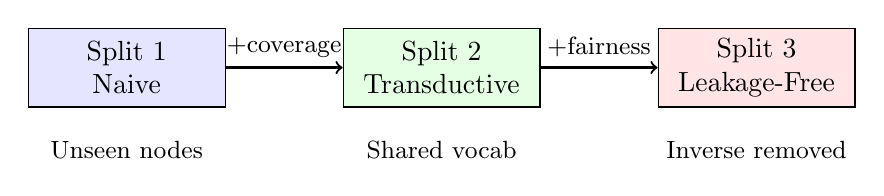
\begin{tikzpicture}[
        box/.style={rectangle, draw, minimum width=2.5cm, minimum height=1cm, align=center},
        arrow/.style={->, thick}
    ]
        % Split 1
        \node[box, fill=blue!10] (s1) at (0,0) {Split 1\\Naive};
        \node[below=0.3cm of s1, font=\small] {Unseen nodes};
        
        % Split 2
        \node[box, fill=green!10] (s2) at (4,0) {Split 2\\Transductive};
        \node[below=0.3cm of s2, font=\small] {Shared vocab};
        
        % Split 3
        \node[box, fill=red!10] (s3) at (8,0) {Split 3\\Leakage-Free};
        \node[below=0.3cm of s3, font=\small] {Inverse removed};
        
        % Arrows showing progression
        \draw[arrow] (s1) -- (s2) node[midway, above, font=\small] {+coverage};
        \draw[arrow] (s2) -- (s3) node[midway, above, font=\small] {+fairness};
    \end{tikzpicture}
    \caption{Progression of Data Splitting Strategies}
\end{figure}

\section{Knowledge Graph Embedding Models}

\subsection{TransE}

TransE \cite{bordes2013translating} models relations as translations in the embedding space.

\textbf{Scoring Function:}
\begin{equation}
    f(h, r, t) = -\|h + r - t\|_{L_2}
\end{equation}

\begin{itemize}
    \item \textbf{Intuition:} Head + Relation $\approx$ Tail in embedding space
    \item \textbf{Strength:} Simple, efficient, handles composition
    \item \textbf{Weakness:} Cannot model \textbf{symmetric relations} (if $h + r = t$, then $t + r \neq h$)
\end{itemize}

\subsection{DistMult}

DistMult \cite{yang2014embedding} uses a bilinear diagonal model for scoring.

\textbf{Scoring Function:}
\begin{equation}
    f(h, r, t) = \langle h, r, t \rangle = \sum_i h_i \cdot r_i \cdot t_i
\end{equation}

\begin{itemize}
    \item \textbf{Intuition:} Trilinear dot product (cosine similarity variant)
    \item \textbf{Strength:} Handles symmetric relations naturally
    \item \textbf{Weakness:} Cannot model \textbf{anti-symmetric}, \textbf{composition}, or \textbf{inverse} relations
\end{itemize}

\subsection{ComplEx}

ComplEx \cite{trouillon2016complex} extends DistMult to complex-valued embeddings.

\textbf{Scoring Function:}
\begin{equation}
    f(h, r, t) = \text{Re}(\langle h, r, \bar{t} \rangle)
\end{equation}

where $\bar{t}$ is the complex conjugate of $t$.

\begin{itemize}
    \item \textbf{Intuition:} Complex-valued embeddings with conjugation
    \item \textbf{Strength:} Handles \textbf{anti-symmetric} relations via conjugation
    \item \textbf{Weakness:} Cannot model \textbf{composition} and \textbf{1-to-N} relations
\end{itemize}

\subsection{RotatE}

RotatE \cite{sun2019rotate} models relations as rotations in complex space.

\textbf{Scoring Function:}
\begin{equation}
    f(h, r, t) = -\|h \circ r - t\|
\end{equation}

where $\circ$ is element-wise rotation in complex plane, $r_i = e^{i\theta_i}$.

\begin{itemize}
    \item \textbf{Intuition:} Relations as \textbf{rotations} in complex space
    \item \textbf{Strength:} Handles \textbf{symmetric}, \textbf{anti-symmetric}, \textbf{inverse}, and \textbf{composition}
    \item \textbf{Theoretical Best:} Most expressive model due to rotation properties
\end{itemize}

\subsection{Model Comparison}

\begin{table}[H]
    \centering
    \caption{Relation Pattern Modeling Capability}
    \begin{tabular}{lcccc}
        \toprule
        \textbf{Pattern} & \textbf{TransE} & \textbf{DistMult} & \textbf{ComplEx} & \textbf{RotatE} \\
        \midrule
        Symmetric & \ding{55} & \ding{51} & \ding{51} & \ding{51} \\
        Anti-symmetric & \ding{51} & \ding{55} & \ding{51} & \ding{51} \\
        Inverse & \ding{51} & \ding{55} & \ding{51} & \ding{51} \\
        Composition & \ding{51} & \ding{55} & \ding{55} & \ding{51} \\
        1-to-N & \ding{55} & \ding{51} & \ding{55} & \ding{51} \\
        \bottomrule
    \end{tabular}
\end{table}

\section{Graph Neural Network Approaches}

\subsection{RGCN (Relational Graph Convolutional Network)}

RGCN \cite{schlichtkrull2018modeling} extends GCN \cite{kipf2016semi} to handle multiple relation types:

\begin{equation}
    h_i^{(l+1)} = \sigma \left( \sum_{r \in R} \sum_{j \in N_i^r} \frac{1}{c_{i,r}} W_r^{(l)} h_j^{(l)} + W_0^{(l)} h_i^{(l)} \right)
\end{equation}

\textbf{Role:} Encoder that produces node embeddings by aggregating neighborhood information across different relation types.

\subsection{RGCN + Decoder Combinations}

\begin{enumerate}
    \item \textbf{RGCN + DistMult:} RGCN encodes nodes, DistMult scores triples
    \item \textbf{RGCN + RotatE:} RGCN with complex-valued features, RotatE decoder
\end{enumerate}

The GNN approach leverages \textbf{graph structure} during encoding, potentially capturing higher-order patterns.

\section{Evaluation Metrics}

\subsection{Mean Reciprocal Rank (MRR)}

\begin{equation}
    MRR = \frac{1}{|Q|} \sum_{i=1}^{|Q|} \frac{1}{\text{rank}_i}
\end{equation}

\textbf{Interpretation:} Average of reciprocal ranks of correct answers. MRR = 1.0 means all correct answers ranked first.

\subsection{Hits@K}

\begin{equation}
    \text{Hits@}K = \frac{|\{q : \text{rank}(q) \leq K\}|}{|Q|}
\end{equation}

\begin{itemize}
    \item \textbf{Hits@1:} Fraction of queries with correct answer in top 1
    \item \textbf{Hits@10:} Fraction with correct answer in top 10
\end{itemize}

\section{Expected Outcomes}

Based on the theoretical properties of models and splitting strategies:

\subsection{Split Type Analysis}

\begin{table}[H]
    \centering
    \caption{Expected Performance by Split Type}
    \begin{tabular}{lccc}
        \toprule
        \textbf{Aspect} & \textbf{Type 1} & \textbf{Type 2} & \textbf{Type 3} \\
        \midrule
        Validation MRR & Low & High & Medium \\
        Unseen Node Issue & Yes & No & No \\
        Inverse Leakage & Yes & Yes & No \\
        True Generalization & Unknown & Inflated & Fair \\
        \bottomrule
    \end{tabular}
\end{table}

\subsection{Model Expectations}

\begin{enumerate}
    \item \textbf{RotatE} should theoretically perform best due to its ability to model all relation patterns
    \item \textbf{TransE} may struggle with symmetric family relations (sibling)
    \item \textbf{DistMult} may struggle with inverse relations (parent $\leftrightarrow$ child)
    \item \textbf{RGCN approaches} should benefit from neighborhood aggregation in dense family clusters
\end{enumerate}

\subsection{Key Insights from Analysis}

\begin{enumerate}
    \item \textbf{Inductive vs Transductive:} Inductive splitting risks unseen nodes; transductive ensures all nodes have embeddings but may allow trivial inverse leakage.
    
    \item \textbf{Inverse Pair Handling:} Critical for family graphs where Father(A,B) often coexists with Son(B,A). Removing these pairs during splitting provides fairer evaluation.
    
    \item \textbf{Model Selection:} RotatE's rotation mechanism makes it theoretically superior for handling the diverse relation patterns in family knowledge graphs.
\end{enumerate}

% ============================================================================
% CONCLUSIONS
% ============================================================================
\newpage
\part{Conclusions}

\section{Summary of Findings}

\subsection{Task 1: Dataset Exploration}

\begin{itemize}
    \item MetaFam is a \textbf{forest of 50 isolated family trees}
    \item Each family spans \textbf{4 generations} with 26-27 members
    \item \textbf{High clustering} (0.73) indicates strong family cohesion
    \item \textbf{No spouse relations} create natural family boundaries
\end{itemize}

\subsection{Task 2: Community Detection}

\begin{itemize}
    \item All algorithms achieved \textbf{near-perfect modularity} ($Q \approx 0.98$)
    \item Communities \textbf{exactly match} the 50 family clusters
    \item \textbf{Louvain and Leiden} produce identical results for sparse graphs
    \item \textbf{No bridge individuals} due to isolated family structure
\end{itemize}

\subsection{Task 3: Rule Mining}

\begin{itemize}
    \item \textbf{5 rules with 100\% confidence} (grandmother, sibling, aunt, symmetry, gender)
    \item \textbf{1 rule with 83\% confidence} (parent/child inverse---incomplete data)
    \item \textbf{2 rules with 0\% confidence} (complex cousin---missing relation types)
    \item Noise analysis: irrelevant predicates cause \textbf{636$\times$ support explosion} but don't affect confidence
\end{itemize}

\subsection{Task 4: Link Prediction}

\begin{itemize}
    \item Three splitting strategies address different evaluation concerns
    \item \textbf{Inverse-leakage removal} is crucial for fair family graph evaluation
    \item \textbf{RotatE} is theoretically optimal for diverse relation patterns
    \item \textbf{RGCN+decoder} approaches leverage graph structure for encoding
\end{itemize}

\section{Interconnections Between Tasks}

\begin{figure}[H]
    \centering
    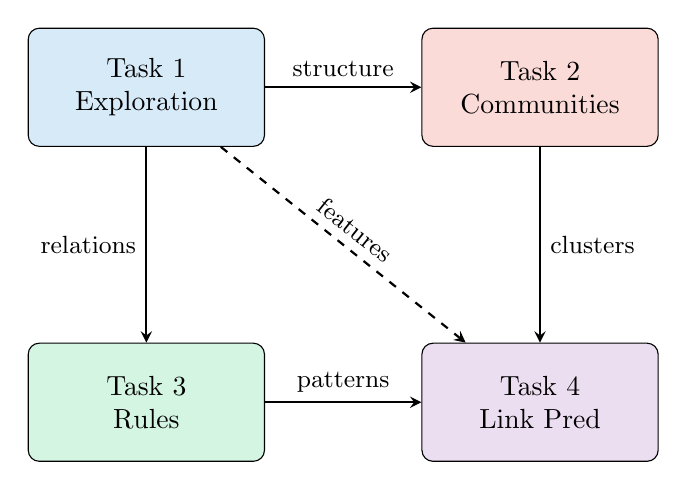
\begin{tikzpicture}[
        task/.style={rectangle, rounded corners, draw, minimum width=3cm, minimum height=1.5cm, align=center},
        arrow/.style={->, thick, >=stealth}
    ]
        \node[task, fill=task1!20] (t1) at (0,4) {Task 1\\Exploration};
        \node[task, fill=task2!20] (t2) at (5,4) {Task 2\\Communities};
        \node[task, fill=task3!20] (t3) at (0,0) {Task 3\\Rules};
        \node[task, fill=task4!20] (t4) at (5,0) {Task 4\\Link Pred};
        
        \draw[arrow] (t1) -- (t2) node[midway, above] {\small structure};
        \draw[arrow] (t1) -- (t3) node[midway, left] {\small relations};
        \draw[arrow] (t2) -- (t4) node[midway, right] {\small clusters};
        \draw[arrow] (t3) -- (t4) node[midway, above] {\small patterns};
        \draw[arrow, dashed] (t1) -- (t4) node[midway, above, sloped] {\small features};
    \end{tikzpicture}
    \caption{Task Dependencies and Information Flow}
\end{figure}

\begin{enumerate}
    \item \textbf{Task 1 $\rightarrow$ Task 2:} Graph structure (50 components) determines community count
    \item \textbf{Task 1 $\rightarrow$ Task 3:} Relation types define possible rules
    \item \textbf{Task 2 $\rightarrow$ Task 4:} Community structure affects link prediction within/across families
    \item \textbf{Task 3 $\rightarrow$ Task 4:} Rules with high confidence can be used as prediction constraints
\end{enumerate}

\section{Technical Recommendations}

\subsection{For Knowledge Graph Analysis}

\begin{enumerate}
    \item Always check for \textbf{connected components} first---they define natural boundaries
    \item \textbf{Gender and generation inference} from relation semantics provides valuable features
    \item High clustering coefficient indicates \textbf{good rule mining potential}
\end{enumerate}

\subsection{For Link Prediction}

\begin{enumerate}
    \item Use \textbf{inverse-leakage removal} for family graphs to avoid overly optimistic metrics
    \item \textbf{Transductive splitting} ensures all entities have embeddings
    \item \textbf{RotatE} is recommended for graphs with diverse relation patterns
    \item Consider \textbf{GNN+decoder} when neighborhood structure is informative
\end{enumerate}

\section{Future Directions}

\begin{enumerate}
    \item \textbf{Add spouse relations:} Would create inter-family bridges and more complex community structure
    \item \textbf{Temporal modeling:} Track relationships over time (births, marriages, deaths)
    \item \textbf{Rule-enhanced link prediction:} Use high-confidence rules as constraints in embedding models
    \item \textbf{Inductive learning:} Develop models that generalize to completely unseen families
\end{enumerate}

% ============================================================================
% APPENDIX
% ============================================================================
\appendix

\section{Project Structure}

\begin{verbatim}
MetaFam-Project/
+-- src/
|   +-- data_loader.py        # Data loading utilities
|   +-- exploration.py        # Task 1: Graph metrics
|   +-- communities.py        # Task 2: Community detection
|   +-- rules.py              # Task 3: Rule validation
|   +-- splitting.py          # Task 4: Data splitting strategies
|   +-- kge_models.py         # Task 4: KGE implementations
|   +-- gnn_models.py         # Task 4: RGCN implementations
|   +-- train_eval.py         # Task 4: Training and evaluation
+-- notebooks/
|   +-- 01_Exploration.ipynb
|   +-- 02_Communities.ipynb
|   +-- 03_Rule_Mining.ipynb
|   +-- 04_Link_Pred.ipynb
+-- data/
|   +-- raw/
|       +-- train.txt
|       +-- test.txt
+-- outputs/
    +-- gephi/                # Graph visualizations
    +-- rules/                # Rule mining results
    +-- splits/               # Generated data splits
    +-- results/              # Model evaluation results
\end{verbatim}

\section{Relation Type Reference}

\begin{longtable}{ll}
    \toprule
    \textbf{Relation} & \textbf{Semantic Meaning} \\
    \midrule
    \endhead
    fatherOf & Head is father of tail \\
    motherOf & Head is mother of tail \\
    sonOf & Head is son of tail \\
    daughterOf & Head is daughter of tail \\
    brotherOf & Head is brother of tail \\
    sisterOf & Head is sister of tail \\
    grandfatherOf & Head is grandfather of tail \\
    grandmotherOf & Head is grandmother of tail \\
    grandsonOf & Head is grandson of tail \\
    granddaughterOf & Head is granddaughter of tail \\
    uncleOf & Head is uncle of tail \\
    auntOf & Head is aunt of tail \\
    nephewOf & Head is nephew of tail \\
    nieceOf & Head is niece of tail \\
    boyCousinOf & Head is male cousin of tail \\
    girlCousinOf & Head is female cousin of tail \\
    \bottomrule
\end{longtable}

\section{Evaluation Metrics Reference}

\begin{table}[H]
    \centering
    \caption{Link Prediction Metrics}
    \begin{tabular}{lll}
        \toprule
        \textbf{Metric} & \textbf{Formula} & \textbf{Range} \\
        \midrule
        MRR & $\frac{1}{|Q|} \sum \frac{1}{\text{rank}_i}$ & [0, 1] \\
        Hits@1 & $\frac{|\text{rank} \leq 1|}{|Q|}$ & [0, 1] \\
        Hits@10 & $\frac{|\text{rank} \leq 10|}{|Q|}$ & [0, 1] \\
        \bottomrule
    \end{tabular}
\end{table}

% ============================================================================
% BIBLIOGRAPHY
% ============================================================================
\newpage
\bibliographystyle{plainnat}
\begin{thebibliography}{99}

\bibitem{girvan2002community}
M.~Girvan and M.~E.~J.~Newman.
\newblock Community structure in social and biological networks.
\newblock {\em Proceedings of the National Academy of Sciences}, 99(12):7821--7826, 2002.

\bibitem{traag2019louvain}
V.~A.~Traag, L.~Waltman, and N.~J.~van Eck.
\newblock From Louvain to Leiden: guaranteeing well-connected communities.
\newblock {\em Scientific Reports}, 9(1):5233, 2019.

\bibitem{bordes2013translating}
A.~Bordes, N.~Usunier, A.~Garcia-Duran, J.~Weston, and O.~Yakhnenko.
\newblock Translating embeddings for modeling multi-relational data.
\newblock In {\em Advances in Neural Information Processing Systems (NeurIPS)}, pages 2787--2795, 2013.

\bibitem{sun2019rotate}
Z.~Sun, Z.-H.~Deng, J.-Y.~Nie, and J.~Tang.
\newblock RotatE: Knowledge graph embedding by relational rotation in complex space.
\newblock In {\em International Conference on Learning Representations (ICLR)}, 2019.

\bibitem{schlichtkrull2018modeling}
M.~Schlichtkrull, T.~N.~Kipf, P.~Bloem, R.~van den Berg, I.~Titov, and M.~Welling.
\newblock Modeling relational data with graph convolutional networks.
\newblock In {\em European Semantic Web Conference (ESWC)}, pages 593--607, 2018.

\bibitem{kipf2016semi}
T.~N.~Kipf and M.~Welling.
\newblock Semi-supervised classification with graph convolutional networks.
\newblock In {\em International Conference on Learning Representations (ICLR)}, 2017.

\bibitem{galarraga2013amie}
L.~Gal{\'a}rraga, C.~Teflioudi, K.~Hose, and F.~Suchanek.
\newblock AMIE: Association rule mining under incomplete evidence in ontological knowledge bases.
\newblock In {\em Proceedings of the 22nd International Conference on World Wide Web (WWW)}, pages 413--422, 2013.

\bibitem{newman2004finding}
M.~E.~J.~Newman and M.~Girvan.
\newblock Finding and evaluating community structure in networks.
\newblock {\em Physical Review E}, 69(2):026113, 2004.

\bibitem{wang2017knowledge}
Q.~Wang, Z.~Mao, B.~Wang, and L.~Guo.
\newblock Knowledge graph embedding: A survey of approaches and applications.
\newblock {\em IEEE Transactions on Knowledge and Data Engineering}, 29(12):2724--2743, 2017.

\end{thebibliography}

\end{document}
